\begin{frame}[noframenumbering]
	\centering
	\huge Performance Results \\ Reactive approach (RA-SPS)
\end{frame}

\begin{frame}{Performance Results : Reactive approach (RA-SPS)}
	\begin{columns}
	\begin{column}{0.6\textwidth}
    	\begin{figure}
		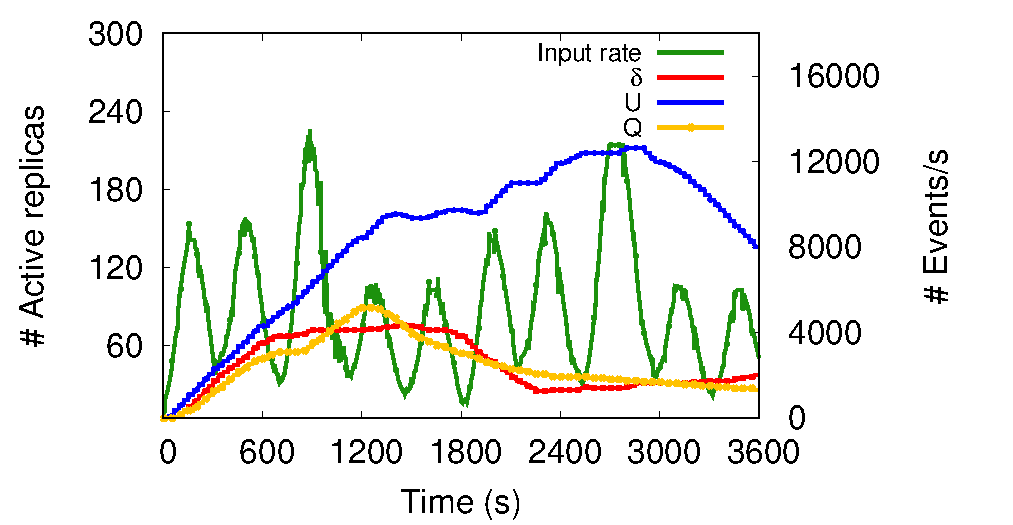
\includegraphics[width=\textwidth]{images/exp/reactive/TwitterLinear-Replicas.pdf}

		\end{figure}
	\end{column}
    \begin{column}{0.55\textwidth}
	    \begin{figure}
		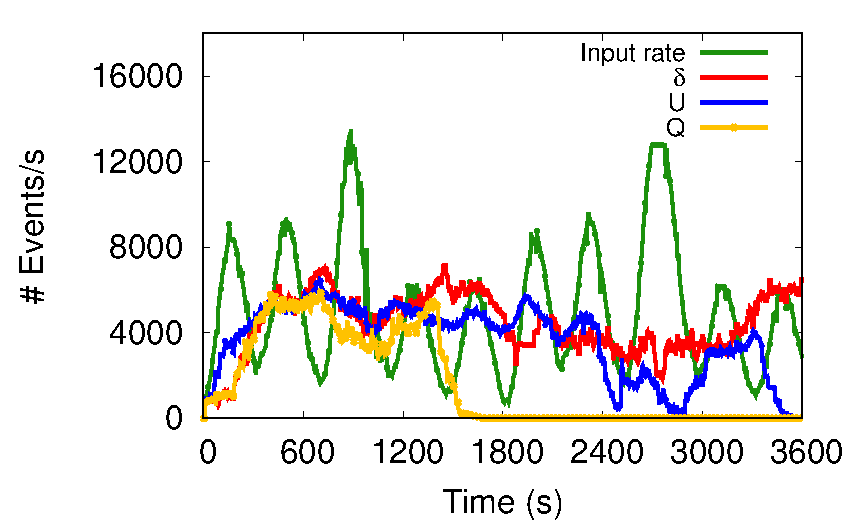
\includegraphics[width=\textwidth]{images/exp/reactive/TwitterLinear-Throughput.pdf}
		\end{figure}
	\end{column}
	\end{columns}
	
	\begin{itemize}
		\item Q queues a lot of events
		\item U overprovides active replicas
		\item $\delta$ is more stable
	\end{itemize}
\end{frame}

\begin{frame}{Performance Results : Reactive approach (RA-SPS)}
	\centering
	
	\begin{table}[!ht]
    \begin{tabular}{|l|llll|}
        \hline
        Metric & \begin{tabular}[c]{@{}l@{}}Saved\\ Nodes\end{tabular} & \begin{tabular}[c]{@{}l@{}}Throughput\\ Degradation\end{tabular} & \begin{tabular}[c]{@{}l@{}}Diff. Proc.\\ Events\end{tabular} & \begin{tabular}[c]{@{}l@{}}Latency\\ (ms)\end{tabular} \\ \hline \hline
        \textbf{$\delta$} & \textbf{0.3996}  & \textbf{0.1092} & \textbf{0.8907} & \textbf{39687.51} \\ \hline
        U        & -0.8934 & 0.2597 & 0.7402 & 23441.39 \\ \hline
        Q        & 0.4975  & 0.6830 & 0.3169 & 28799.60 \\ \hline
        \end{tabular}
    \end{table}
    
    \begin{itemize}
    	\item $\delta$ process more events that U and Q
    	\item $\delta$ does not consider dependency, so there is cascading problem
    \end{itemize}
\end{frame}

